\documentclass[aspectratio=169]{beamer} % [mathserif]
\usepackage{amsmath}
\usepackage{graphicx}
\usepackage{subfigure}
\usepackage{wrapfig}
\usepackage{booktabs}
\usepackage{hyperref}
\usepackage{media9}
\usepackage{xcolor}
%\usepackage{enumitem}
% \usepackage{pgfplots}
% \pgfplotsset{compat=1.18}
% \usepgfplotslibrary{dateplot}
% \usepackage{tipa}
% \usepackage{epstopdf} % this is needed for windows Texworks
\usepackage[absolute,overlay]{textpos} % ,showboxes

\setlength{\TPHorizModule}{1in}
\TPVertModule=\TPHorizModule

\DeclareGraphicsExtensions{.eps}

\usetheme{Marburg}
% \usetheme{Berkeley}
% \usecolortheme{rose}
\definecolor{naublue}{HTML}{002454}
\definecolor{nauyellow}{HTML}{FAC01A}
%\setbeamercolor{structure}{bg=nauyellow, fg=naublue}
\setbeamercolor{palette primary}{bg=nauyellow, fg=naublue}
\setbeamercolor{palette secondary}{bg=nauyellow, fg=naublue}
%%%% See https://en.wikibooks.org/wiki/LaTeX/Presentations#User-defined_themes
% \setbeamercolor{alerted text}{fg=orange}
% \setbeamercolor{background canvas}{bg=white}
% \setbeamercolor{block body alerted}{bg=normal text.bg!90!black}
% \setbeamercolor{block body}{bg=normal text.bg!90!black}
% \setbeamercolor{block body example}{bg=normal text.bg!90!black}
% \setbeamercolor{block title alerted}{use={normal text,alerted text},fg=alerted text.fg!75!normal text.fg,bg=normal text.bg!75!black}
% \setbeamercolor{block title}{bg=blue}
% \setbeamercolor{block title example}{use={normal text,example text},fg=example text.fg!75!normal text.fg,bg=normal text.bg!75!black}
% \setbeamercolor{fine separation line}{}
\setbeamercolor{frametitle}{fg=naublue}
% \setbeamercolor{item projected}{fg=black}
% \setbeamercolor{normal text}{bg=black,fg=yellow}
% \setbeamercolor{palette sidebar primary}{use=normal text,fg=normal text.fg}
\setbeamercolor{palette sidebar primary}{bg=naublue, fg=nauyellow}
% \setbeamercolor{palette sidebar quaternary}{use=structure,fg=structure.fg}
% \setbeamercolor{palette sidebar secondary}{use=structure,fg=structure.fg}
% \setbeamercolor{palette sidebar tertiary}{use=normal text,fg=normal text.fg}
\setbeamercolor{section in sidebar}{fg=nauyellow, bg=naublue}
\setbeamercolor{section in sidebar shaded}{fg=white}
% \setbeamercolor{separation line}{}
% \setbeamercolor{sidebar}{bg=red}
% \setbeamercolor{sidebar}{parent=palette primary}
% \setbeamercolor{structure}{bg=black, fg=green}
% \setbeamercolor{subsection in sidebar}{fg=brown}
% \setbeamercolor{subsection in sidebar shaded}{fg=grey}
\setbeamercolor{title}{fg=naublue}
% \setbeamercolor{titlelike}{fg=brown}

% \usepackage[latin1]{inputenc}

%%%% See https://en.wikibooks.org/wiki/LaTeX/Presentations#Title_page_and_author_information
\title[INF632 (EE499/EE599)]{Wearable Technologies and Applications\\(Wearable Informatics)} %
\author{Winfree}
\date{Lecture 10}
%\institute{Northern Arizona University}

%\logo{\includegraphics[width=.5in]{figures/logo}}
% \setbeameroption{show notes on second screen}

\begin{document}
	\maketitle


% \section[Outline]{}
% \frame{\tableofcontents}

\section{{\em The} Discussion}
	\begin{frame}
		\frametitle{Pre-Discussion}
		At this point, you have:
		\begin{itemize}
			\item Introduced your project
			\begin{itemize}
				\item With a background review, previous literature / prior work
				\item Which has allowed you to frame the importance of your work
			\end{itemize}
			\item Detailed your hardware design and methods
			\begin{itemize}
				\item In this case, you have probably included schematics and descriptions of what you have built
				\item And, what steps you took in your study
			\end{itemize}
			\item Provided the results
			\begin{itemize}
				\item But the results section is typically very dry
				\item It {\em should} be very dry!
				\item In the results is {\em not} where you discuss the interpretation or meaning of your results ... that goes into the discussion section
			\end{itemize}
		\end{itemize}
	\end{frame}

	\subsection{Purpose and Structure}
	\begin{frame}
		\frametitle{Purpose}
		There are five key goals of the discussion section
		\begin{columns}
			\begin{column}{.25\linewidth}
			\begin{enumerate}
				\item Interpretation
				\item Context
				\item Limitations
				\item Implications
				\item Next steps
			\end{enumerate}
			\end{column}
			\begin{column}{.75\linewidth}
				~
			\end{column}
		\end{columns}
	\end{frame}

	\begin{frame}
		\frametitle{Structure}
		\begin{columns}
			\begin{column}{.25\linewidth}
				Five key goals
				\begin{enumerate}
					\item Interpretation
					\item Context
					\item Limitations
					\item Implications
					\item Next steps
				\end{enumerate}
			\end{column}
			\begin{column}{.75\linewidth}
				Make it flow
				% \begingroup
				% \renewcommand\labelitemi{}
				\begin{itemize}%[label={}]
					\item Concise summary of main findings% $\rightarrow$
					\item Interpretation / Meaning% $\rightarrow$
					\item Comparison to prior work% $\rightarrow$
					\item Limitations (those with impact)% $\rightarrow$
					\item Practical implications% $\rightarrow$
					\item Future work / Concluding statement
				\end{itemize}
				% \endgroup
			\end{column}
		\end{columns}
	\end{frame}

\section{Ask Yourself}
	\begin{frame}
	\frametitle{Ask Yourself}
		But there is more to it than just hitting five bullet points with six parts of the story.

		Here are a few tips, or considerations, in writing a clear and convincing discussion section.

		Note, much of this will feel like stuff that should have been considered before starting the project or study.  Fair point, and yes, much of this is.  But not all of this will be obvious ahead of time, or even practical to address at that time.
	\end{frame}

	\subsection{Results vs Interpretation}
	\begin{frame}
	\frametitle{Results vs Interpretation}
	\begin{columns}
			\begin{column}{.25\linewidth}
				{\bf Distinguishing results vs interpretation:}
				\begin{itemize}
					\item What does the data directly show?
					\item What are you inferring?
					\item Avoid overstating causality!
				\end{itemize}
			\end{column}
			\begin{column}{.75\linewidth}
				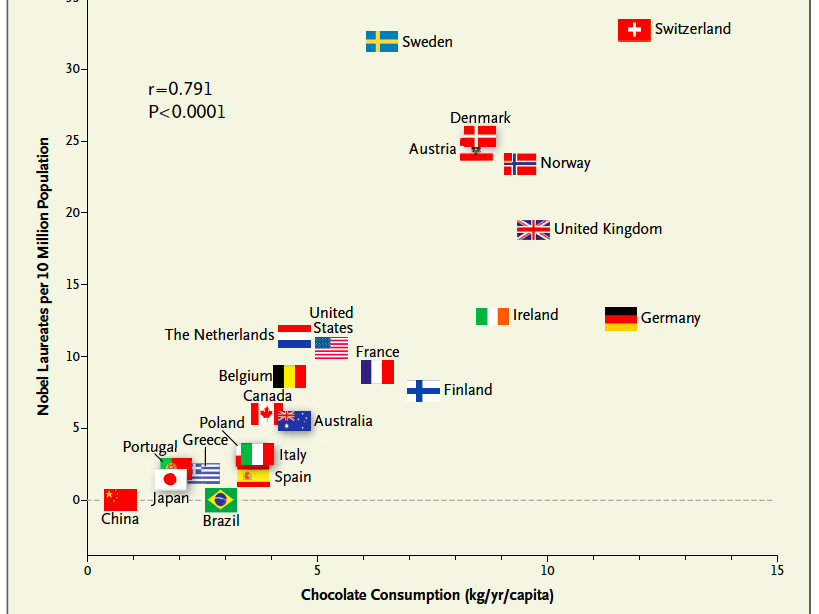
\includegraphics[width=1\linewidth]{figures/chocloate.png}
			\end{column}
		\end{columns}
		
	\end{frame}

	\subsection{Link Analyses to Claims}
	\begin{frame}
	\frametitle{Link Analyses to Claims}
		{\bf Linking analyses to claims:}
		\begin{itemize}
			\item Map each major claim to the supporting analysis/figure and quantify uncertainty.
			\item Make use of confidence intervals, effect sizes, p-values where relevant.
		\end{itemize}
	\end{frame}

	\subsection{Significance}
	\begin{frame}
	\frametitle{Significance}
		{\bf Effect sizes and practical significance:}
		\begin{itemize}
			\item Explain why small statistically significant differences may be meaningless for real-world wearable use.
			\item Are there clinically significant thresholds that should be considered?
		\end{itemize}
	\end{frame}

	\subsection{Uncertainty}
	\begin{frame}
	\frametitle{Uncertainty}
		{\bf Uncertainty and robustness checks:}
		\begin{itemize}
			\item Consider sensitivity analyses:
				\begin{itemize}
					\item What happens when you vary assumptions, inputs, model choices, or processing steps?
					\item If small, plausible changes produce large shifts in conclusions, those conclusions are fragile.
					\item Sensors and prepossessing choices (filter cutoffs, interpolation) can strongly affect derived measures.
					\item Model hyper-parameters, feature selection, window sizes, and labeling methods influence performance.
					\item Participant sampling, missing data handling, and ground-truth quality can introduce bias.
				\end{itemize}
			\item Did you perform cross-validation?
			\item Do error bars in your plots suggest a dependence in your variables is there?
			\item reproducibility notes.
		\end{itemize}
	\end{frame}

	\subsection{Limitations}
	\begin{frame}
	\frametitle{Limitations}
		{\bf Limitations (technical and experimental):}
		\begin{itemize}
			\item What limitations do your sensors have?
			\item Is there sampling bias? Not just participants, but sampling rate too.
			\item How does calibration of your sensors or outputs factor in here?
			\item Is there a possibility of latency issues?  Do they matter in your application?  Did you address them?
			\item Do you have an appropriately diverse (age, gender, ethnicity) participant pool?
			\item {\bf What are your algorithm assumptions?}
		\end{itemize}
	\end{frame}

	\subsection{Validity}
	\begin{frame}
	\frametitle{Validity}
		{\bf Confounding, bias, and threats to validity:}
		\begin{itemize}
			\item What potential is there for measurement error?
			\item Do you have any selection bias
			\item We talked about over fitting earlier - have you tested for this?
			\item If you are training a model on ground-truth labels or measures, how confident are you with that ground truth?
		\end{itemize}
	\end{frame}

	\subsection{Failures}
	\begin{frame}
	\frametitle{Failures}
		{\bf How to discuss failures and negative results:}
		\begin{itemize}
			\item Be transparent!  Yes, there is value to papers that say ``this didn't work as expected.''
			\item Try to explain the root causes of these results.
			\item What did you learn from these results?  How do these results contribute to the field of science? Do these results inform future efforts by others?
			\item What change to your hardware, software, study design, or even analysis should be considered for ``next time''?
		\end{itemize}
	\end{frame}

	\subsection{Prior Work}
	\begin{frame}
	\frametitle{Prior Work}
		{\bf When relating your work to prior work:}
		\begin{itemize}
			\item Be concise.
			\item Make {\em fair} comparisons - explain why differences exist (methods, sensors, populations).
			\item Science advances through thoughtful critique — pointing out limitations, differences, and improvements respectfully and constructively, not through harsh or dismissive attacks.
		\end{itemize}
	\end{frame}

	\subsection{Visuals}
	\begin{frame}
	\frametitle{Visuals}
		{\bf Visual presentation of results:} When working on your discussion, reflect on the results and ask:
		\begin{itemize}
			\item Did you choose the right plots?
			\item Are those plots labeled for clarity?
			\item Do your scales mislead the reader?  Could they?
		\end{itemize}
	\end{frame}

	\subsection{Writing Style}
	\begin{frame}
	\frametitle{Writing Style}
		{\bf Writing style and tone:} How you write is as important as the content.
		\begin{itemize}
			\item Are you being concise?
			\item Are you being honest?
			\item Do you have defensible claims?
			\item Avoid hedging that obscures meaning or implies stretch conclusions.
			\item Avoid jargon!  And for that matter, acronyms.
			\begin{itemize}
				\item Acronyms, by and large, are not universal.
				\item Consider how those acronyms might have different common meanings for others.
				\item Defining acronyms doesn't not absolve you of this issue.
				\item Limit not just your use, including how many you define.
				\item Always ask yourself if the acronym actually improves your writing, or if it instead distracts the reader from the point you are trying to make.
			\end{itemize}
		\end{itemize}
	\end{frame}

	\subsection{Ethics}
	\begin{frame}
	\frametitle{Ethics}
		{\bf Ethical and user-centered implications:} Science is morally neutral, it doesn't care, but you should. 
		\begin{itemize}
			\item Does your study present privacy concerns?
			\item Are there real-world deployment concerns?
			\item Could your results be easily misinterpreted in an ethically or morally inappropriate way?
		\end{itemize}
	\end{frame}

	\subsection{Reproducibility}
	\begin{frame}
	\frametitle{Reproducibility}
		{\bf Reproducibility and data or code sharing:} 
		\begin{itemize}
			\item What can you include as supplementary materials?
			\item If you are sharing your code, have you practiced good documentation?
		\end{itemize}
	\end{frame}

	\subsection{Closing Takeaways}
	\begin{frame}
	\frametitle{Closing Takeaways}
		{\bf Practical engineering takeaways and closing statements:} 
		\begin{itemize}
			\item How should your results inform product design?
			\item Or product decisions?
			\item Or more generally, next experiments?\\{\em (the science is never done)}
			\item If you wanted your readers to remember one thing from your paper, what would it be?  Did you get that when you read your discussion?  Restate your point as needed...
		\end{itemize}
	\end{frame}

\section{TLDR;}
	\begin{frame}
		\frametitle{TLDR;}
			{\bf Honesty is always better than Hype:} clear limits and realistic claims increase your paper's (your) credibility.

			{\bf Always tie your claims to your evidence:} point to the exact analysis or figure that supports each statement.

			{\bf Quantify uncertainty and the practical impact, do not just report p-values.}

			{\bf Be explicit about your assumptions and how they affect conclusions.} Model assumptions included.

			{\bf Failure is informative:} explain why something didn't work, that is still valuable science and engineering.

			{\bf Clarity in visuals (plots, tables, diagrams) and writing wins:} A correct, but unclear paper fails to communicate the thoughts.  No one will see your genius if you can't communicate it to them.

			{\bf Consider the audience:} Who will be reading your paper; what researchers, clinicians, or designers need to know what you are sharing and how will they likely use the results?
	\end{frame}

\section{In Class Discussion Time}
	\begin{frame}
		\begin{columns}
			\begin{column}{.4\linewidth}
				In 10 minutes and in pairs, identify:
				\begin{enumerate}
					\item 3 strengths
					\item 3 weaknesses
					\item 2 unstated assumptions
					\item Bonus: Reword a sentence to strengthen the claim.
				\end{enumerate}
				After 10 minutes, we will regroup and report back, then move on to the next paper.
			\end{column}
			\begin{column}{.6\linewidth}
				Ask yourself
				\begin{enumerate}
					\item Does each main claim cite a specific result or figure?
					\item Is uncertainty reported?
					\item Are the limitations clearly stated and their impact discussed?
					\item Are alternative explanations and confounding variables considered?
					\item Is the practical significance discussed in context of real-world use?
					\item Are the methods or thresholds that impact interpretation explained, or mentioned?
					\item Is the language appropriately cautious?  Or have the authors maybe overstated causality?
				\end{enumerate}
			\end{column}
		\end{columns}
	\end{frame}
\end{document}
